\documentclass[crop,border=7pt]{standalone}
\usepackage{tikz}
\usetikzlibrary{calc,patterns}
\begin{document}
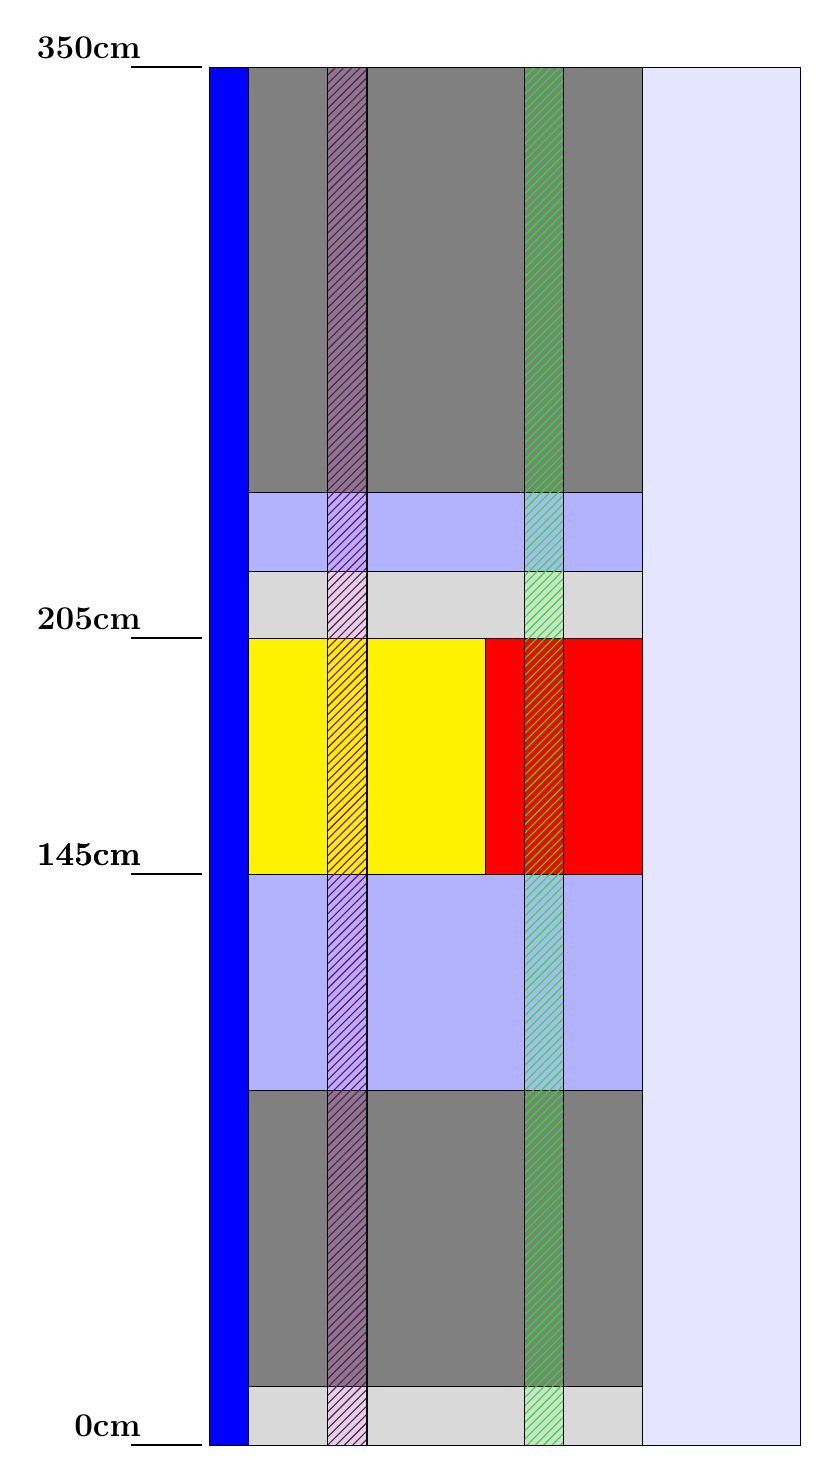
\begin{tikzpicture}[scale=0.5]

%PROFILE REACTOR
\filldraw[fill=blue!10, draw=black] (0,0) rectangle (15,35);

\filldraw[fill=blue, draw=black] (0,0) rectangle (1,35);
\filldraw[fill=gray, draw=black] (1,0) rectangle (11,14.5);
\filldraw[fill=gray!30, draw=black] (1,0) rectangle (11,1.5);
\filldraw[fill=blue!30, draw=black] (1,9) rectangle (11,14.5);
\filldraw[fill=yellow] (1,14.5) rectangle (7,20.5);
\filldraw[fill=gray, draw=black] (1,20.5) rectangle (11,35);
\filldraw[fill=red] (7,14.5) rectangle (11,20.5);

\filldraw[fill=gray!30, draw=black] (1,20.5) rectangle (11,22.2);

\filldraw[fill=blue!30, draw=black] (1,22.2) rectangle (11,24.2);

%rods
\draw[pattern=north east lines,pattern color=violet] (3,0) rectangle (4,35);

\draw[pattern=north east lines,pattern color=green] (8,0) rectangle (9,35);

%%%%%%%%%%%%%%%%%%%%%%%%%%%%

%\draw (0,0) -- (4,0);
\draw[black, thick] (-0.2,0) -- (-2,0);
\draw[black] (-1.5,0.5) node[anchor=east] {\large \textbf{0cm}};
%%%%%%%%%%%
\draw[black, thick] (-0.2,14.5) -- (-2,14.5);
\draw[black] (-1.5,15) node[anchor=east] {\large \textbf{145cm}};
%%%%%%%%%%5
\draw[black, thick] (-0.2,14.5) -- (-2,14.5);
\draw[black] (-1.5,15) node[anchor=east] {\large \textbf{145cm}};
%%%%%%%%%%%%%%%%%%%%
\draw[black, thick] (-0.2,20.5) -- (-2,20.5);
\draw[black] (-1.5,21) node[anchor=east] {\large \textbf{205cm}};
%%%%%%%%%%%%%%%%
\draw[black, thick] (-0.2,35) -- (-2,35);
\draw[black] (-1.5,35.5) node[anchor=east] {\large \textbf{350cm}};
\end{tikzpicture}
\end{document}